\documentclass{article}
\usepackage{graphicx}
\begin{document}

\newpage
\title{DBMS Mini Project}
\author{Vaibhav Nayak}
\date{12 JAN 2023}
This is the first paragraph on the front page.\par
This is the second paragraph on the front page.\par

\newpage
\section{Acknowledgement to the teacher}
This one is for all my friends\par
This one is for my doggo\par

\newpage
\section{Table of Contents}
\begin{itemize}
\item 1. Introduction
\item 2. Literature Review
\item 3. Methodology
\item 4. Results
\item 5. Discussion
\item 6. Conclusion
\item 7. References
\end{itemize}

\newpage
\title{Introduction}
\begin{abstract}
Overview of the Report
\end{abstract}
\begin{figure}[h!]
\centering
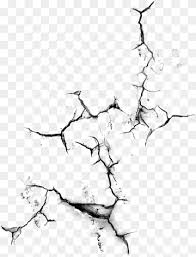
\includegraphics[width=0.5\textwidth]{figure1.png}
\caption{Figure 1: Sample Figure}
\end{figure}
\begin{figure}[h!]
\centering

\includegraphics[width=0.5\textwidth]{figure2.png}
\caption{Figure 2: Not a Sample Figure}
\end{figure}
\begin{thebibliography}{100}
\bibitem{0}
Author, A. (Year). Title of the paper. Journal Name, Volume(Issue), pages.
\bibitem{1}
Author, A. (Year). Title of the paper. Journal Name, Volume(Issue), pages.
\end{thebibliography}

\end{document}